\documentclass[usenames,dvipsnames,letterpaper,landscape,final]{slides}

\def\fileHome{.}
\def\icons{\fileHome/icons}

\input mySlideStyle2019-1.tex
\def\myfboxBlack#1{\fboxrule2pt\fbox{$\ds#1$}}
\newcommand\topSeparatorHeading[1]{\noPagetrue\begin{myslide}\headingline\vbox to5.5in{%
\vfil\begin{center}{{\large\myfboxBlack{\myfboxBlack{%
\text{\ \ \bf\Blue{\begin{tabular}{c}#1\end{tabular}\ \ }}}}}}%
\end{center}\vfil}\end{myslide}\noPagefalse}

\usepackage{multirow}
\usepackage{enumitem}
\usepackage[ruled,vlined]{algorithm2e}
%\usepackage{wallpaper}
		  \usepackage{mathtools}

\newcounter{outlineNumber}\setcounter{outlineNumber}{0}
\def\outno{\stepcounter{outlineNumber}\Blue{\theoutlineNumber. }}

\definecolor{boxColor}{rgb}{.4, .05, .2}

%------------------------------------------------------------------------------
\tikzset{cross/.style={cross out, draw=black, minimum size=2*(#1-\pgflinewidth), inner sep=0pt, outer sep=0pt},cross/.default={1pt}}

\renewcommand\floatpagefraction{0}
\renewcommand\textfraction{0}
\renewcommand\topfraction{1}
\renewcommand\bottomfraction{1}
\setcounter{topnumber}{10}
\setcounter{bottomnumber}{10}
\setcounter{totalnumber}{10}

\def\picWidth#1#2{\includegraphics[clip=true,keepaspectratio=true,width=#1]{#2}}
\def\picHeight#1#2{\includegraphics[clip=true,keepaspectratio=true,height=#1]{#2}}
\def\picWidthHeight#1#2#3{\includegraphics[clip=true,width=#1,height=#2]{#3}}

%\let\itemOld=\item
%\def\item{\parskip=0pt\itemsep=0pt\itemOld}


\begin{document}

% ===========================================

\begin{myslide}
\headingline
		  %\vspace*{-30pt}
		  {\bf\Large\begin{center}
					 Simulation of Partial Melting Mantle
		  \end{center}}

\vfill

\begin{center}{\obeylines
Chenyu Tian
\bigskip
%		  {\it\OliveGreen{CSEM} 
%		  \Blue{\it Oden Institute}}
%\BurntOrange{The University of Texas at Austin}}
	  {CSEM, Oden Institute}
The University of Texas at Austin}
\end{center}

\vfill

{\tiny\begin{center}
					 Todd Arbogast, Oden Institute \& Mathematics, University of Texas at Austin\\
Marc A. Hesse, Oden Institute \& Geosciences, University of Texas at Austin\\
		  \end{center}}

		  \vspace*{40pt}

\end{myslide}

% ===========================================

\begin{myslide}
\heading{Introduction}

\Oblue{Mantle melting}:
\begin{nlist}
\item Mantle melting is a crucial geophysical process in lithospheric evolution and plate tectonics.
\item Geophysical evidence indicates that the asthenosphere is often partially molten.
\item A thorough understanding of partial melting is fundamental to comprehending the dynamics of 
magmatism. 
\end{nlist}

\vspace{20pt}

\Oblue{Partial Melting}:
		  \begin{nlist}
		  \item Modeled as a two-phase flow framework.
		  \item Coupled with complicated chemical interactions.
		  \item Compaction is essential in deciding melt extraction and segregation.
		  \end{nlist}

\vspace{20pt}

		  {\Oorange{Challenge}}:
\begin{nlist}
\item Degenercy caused by no-melt regions poses mathematical and numerical difficulties.  
\end{nlist}

\end{myslide}

% ===========================================

\begin{myslide}
\heading{New framework}

\Oblue{Physical Model}:
\begin{nlist}
\item A degenerate two-phase Darcy–Stokes system describing the coupled interaction
between the solid matrix and the interstitial melt.
\item A nonlinear system governing the transport of chemical species and thermal
energy.
\item A eutectic phase relation characterizing the melting processes and connecting
the transport and static mechanical system through enthalpy method.
\end{nlist}

\vspace{20pt}
\Oblue{Numerical Methods}:
\begin{nlist}
\item $H(\text{div})$-and $H^1$- conforming mixed finite element spaces for Darcy and Stokes subproblems.
\item A more versatile and flexible multilevel WENO weighting scheme to address the nonlinear transport of chemical species and energy in the 
presence of porous media.
\end{nlist}

\end{myslide}

% ===========================================

\separatorHeading{\outno Physical Model}

\begin{myslide}
\heading{Static Mechanical System}

		  \Oblue{Darcy-Stokes system}:
\begin{alignat}{2}
    \label{eq:darcy}
		  &\phi_l (\mathbf{v}_l - \mathbf{v}_s)
		  + \frac{k_{\phi_l}}{\mu_l}(\nabla p_l - \rho_f\mathbf{g})
	    &&= 0,\\
	\label{eq:continuous}
		  &\nabla \cdot (\phi_l\mathbf{v}_l + \phi_s\mathbf{v}_s) &&=0,\\
	\label{eq:stokes}
		  &\nabla\bar p - \nabla \cdot \pmb{\tau}(\mathbf{v}_s) + \overline{\rho}\mathbf{g}&&= 0,\\
	\label{eq:compaction}
		  &\mu_s\nabla \cdot \mathbf{v}_s - \phi_l(p_l - p_s) &&=0, 
\end{alignat}

		  \vspace{20pt}
		  \Oblue{Deviatoric stress}: 
\begin{equation}\label{eq:deviatoricstress}
		  \pmb{\tau}(\mathbf{v}_s)
		  = 2\mu_s\phi_s\big(\mathcal{D} \mathbf{v}_s - \tfrac{1}{3}\nabla \cdot \mathbf{v}_s \mathbf{I}\big),
\end{equation}

\end{myslide}

% ===========================================

\begin{myslide}
\heading{Transport of Chemical Species}

\Oblue{Transport of chemical species}:
\begin{equation} \label{eq:specietransport}
		  \frac{\partial \overline{\rho c_{i}}}{\partial t} + \nabla \cdot \big( \overline{\rho c_{i} \mathbf{v}} - \phi_l \rho_l \mathcal{D}_{i,l} \nabla c_{i,l} \big) = 0,
\end{equation}

\vspace{20pt}

\Oorange{Phase averaged quantities}:
\begin{equation}
\overline{\rho c_i} = \sum_{j\in \{s,l\}} \phi_j \rho_j c_{i,j}, \quad 
\overline{\rho c_i \mathbf{v}} = \sum_{j\in \{s,l\}} \phi_j \rho_j c_{i,j} \mathbf{v}_j.
\end{equation}

\Oorange{Effective Velocity}:

\begin{equation}
\label{eq:effectivevel}
		  \overline{c_{i}\bold{v}} = \phi_s \bold{v}_s c_{i,s} + \phi_l \bold{v}_l c_{i,l} = 
		  \bigg( \frac{\phi_l \bold{v}_l + D\phi_s \bold{v}_s}{\phi_l + \phi_s D} \bigg) \overline{c}_i.
\end{equation}

\vspace{20pt}

\Oblue{Reformation}:
\begin{equation}\label{eq:effectivetransportspecie}
		  \frac{\partial C}{\partial t} = 
		  \nabla \cdot (\mathbf{v}_{\text{eff}} C - \phi_l \mathcal{D}_l \nabla c_l)
		  = 0
\end{equation}

\end{myslide}

% ===========================================
\begin{myslide}
\heading{Transport of Energy}
\Oblue{Specific internal energy formulation}:
\begin{equation}\label{eq:energybalanceinternalenergy}
\frac{\partial \overline{\rho u}}{\partial t} + \nabla \cdot \overline{\rho u \mathbf{v}} = 
		  \overline{\rho \mathcal{Q}} + \nabla \cdot \overline{K} \nabla T + \nabla \cdot \overline{\pmb{\sigma} \cdot \mathbf{v}} +
		  \overline{\rho \mathbf{v}} \cdot \mathbf{g},
\end{equation}
where $\overline{K} = \phi_l K_l + \phi_s K_s$ is the phase averaged thermal conductivity.

\vspace{20pt}

\Oblue{Temperature formulation}:
\begin{equation}\label{eq:normalizedenthalpy}
		  \frac{\partial \overline{H}}{\partial t} + \nabla \cdot (\overline{\mathbf{v}} T) = 
		  \frac{L}{c_p} \nabla \cdot (\phi_s \mathbf{v}_s) + \kappa \nabla^2 T + 
		  \frac{\alpha_\rho}{c_p} T \overline{\mathbf{v}} \cdot \mathbf{g},
\end{equation}

\vspace{20pt}

\Oorange{Specific enthalpy}:
\begin{equation}\label{eq:specificenthalpy}
		  h_i = u_i + p_i\tilde{V}_i = u_i + P/\rho_i,
\end{equation}

\vspace{20pt}

\Oorange{Bulk specific enthalpy}:
\begin{equation}
\overline{H} = \overline{\rho h}/\rho c_p = \overline{h}/c_p
\end{equation} 


\end{myslide}

% ===========================================

\begin{myslide}
\heading{Phase transition}
\centering\small
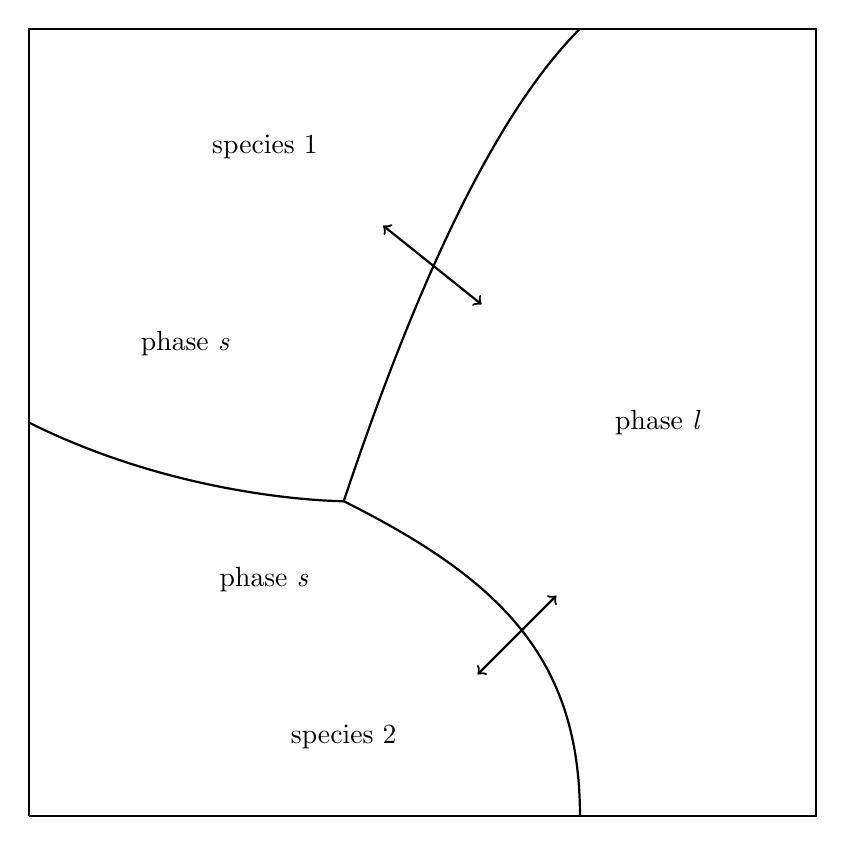
\begin{tikzpicture}[scale=1.0]
    \draw [thick] (0,0) -- (10,0) -- (10,10) -- (0,10) -- (0,0);
    \draw [thick] (0,5) .. controls (2,4) and (4,4) .. (4,4);
    \draw [thick] (4,4) .. controls (5,7) and (6,9) .. (7,10);
    \draw [thick] (4,4) .. controls (6,3) and (7,2) .. (7,0);
    
    %\draw (4,1) node {$\rho_2=c_{2,2}$};
    %\draw (3,8.5) node {$\rho_1=c_{1,1}=c_s$};
    %\draw (7.5,6) node {$c_{1,f}=c_{f}$};
    %\draw (7.8,3) node {$c_{2,f}$};

    \draw (4,1) node {species 2};
    \draw (3,8.5) node {species 1};

    \draw [thick, <->] (5.7,1.8) -- (6.7,2.8);
    \draw [thick, <->] (4.5,7.5) -- (5.75,6.5);
    %\draw [thick, <->] (7.8,3.8) -- (7.8,5.2);
    
		  \draw (2,6) node {phase \textit{s}};
		  \draw (3,3) node {phase \textit{s}};
		  \draw (8,5) node {phase \textit{l}};
\end{tikzpicture}

\end{myslide}

% ===========================================
\begin{myslide}
\heading{Eutectic phase behavior}

\Oblue{Phase diagram}:

\begin{center}
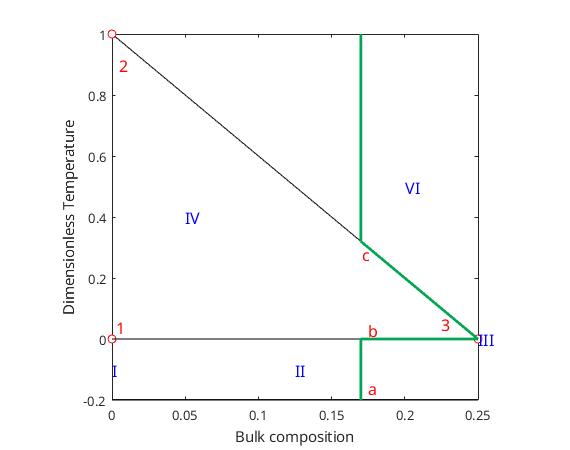
\includegraphics[width=10cm,height=7cm]{../formal/chapters/pics/zoom_eutectic.png}
\end{center}

\vspace{20pt}

\Oblue{Enthalpy-Composition diagram}:

\begin{center}

\includegraphics[width=10cm,height=7cm]{../formal/chapters/pics/HC.png}
\end{center}

\end{myslide}
% ===========================================

% ===========================================

\separatorHeading{\outno Numerical Methods}

\begin{myslide}
\heading{Scaled Formulation}
\Oblue{Scaled variables}: 
\begin{equation}\label{eq:scaledVariables}
		  \tilde{\mathbf{v}}_r = \phi^{-\Theta}\mathbf{v}_r
	\quad\text{and}\quad
	\tilde{q}_l = \phi^{1/2}q_l,
\end{equation}
\Oblue{Scaled Equations}:
\begin{alignat}{2}
\label{eq:darcy_flow_sc}
		  &\tilde{\mathbf{v}}_r
		  + \frac{k_0\phi^{1+\Theta}}{\mu_l}\nabla(\phi^{-1/2}\tilde{q}_l)
        &&= 0,\\
\label{eq:consMass_flow_sc}
		  &\mu_s\phi^{-1/2}\nabla \cdot(\phi^{1+\Theta}\tilde{\mathbf{v}}_r)
        + \frac{1}{1-\phi}(\tilde{q}_l - \phi^{1/2}q) &&=0,\\
\label{eq:stokes_flow_sc}
		  &\nabla q - \nabla \cdot \tau(\mathbf{v}_s) &&= -(1-\phi)\rho_r \mathbf{g},\\
\label{eq:compaction_flow_sc}
		  &\mu_s\nabla \cdot \mathbf{v}_s
        - \frac{\phi^{1/2}}{1-\phi}(\tilde{q}_l - \phi^{1/2}q) &&=0,
\end{alignat}

\vspace{20pt}

\Oblue{Well-defined condition}:
\begin{equation}\label{eq:phiboundness}
		  \phi^{\Theta - 1/2} \nabla \phi \in (L^{\infty}(\Omega))^2.
\end{equation}

\end{myslide}

\begin{myslide}
\heading{Scaled Hilbert Space}
Let
\begin{equation}\label{eq:scaledHspace}
		  H_{\phi}(\text{div}; \Omega) = \Big\{ \mathbf{v} 
		  \in (L^2(\Omega))^2: \phi^{-1/2}\nabla \cdot (\phi^{1+\Theta} \mathbf{v})
		  \in L^2(\Omega) \Big\}.
\end{equation}
This is a Hilbert space equipped with the inner product
\begin{equation}\label{eq:scaledinnerp}
		  (\mathbf{u}, \mathbf{v})_{H_\phi(\text{div};\Omega)} = 
		  (\mathbf{u}, \mathbf{v}) + 
		  (\phi^{-1/2} \nabla \cdot (\phi^{1+\Theta}\mathbf{u}), \phi^{-1/2} \nabla \cdot (\phi^{1+\Theta}\mathbf{v})).
\end{equation}
The normal trace on $\partial \Omega$ is well-defined by
		  \begin{equation}\label{eq:scaledtraceoperator}
		  \langle \phi^{1/2+\Theta} \mathbf{v}\cdot \pmb{\nu}, \psi \rangle = \big(\mathbf{v}, \phi^{1+\Theta}\nabla(\phi^{-1/2}\psi)\big) + 
		  \big(\phi^{-1/2}\nabla \cdot (\phi^{1+\Theta}\mathbf{v}),\psi \big), \quad \forall \psi \in H^1(\Omega),
\end{equation}
		  using~\eqref{eq:phiboundness}, moreover,
\begin{equation}\label{eq:tracescaled}
		  \norm{\phi^{1/2+\Theta}\mathbf{v}\cdot \pmb{\nu}}_{H^{-1/2}(\partial \Omega)} < C_{\Omega} \Big\{ \norm{\mathbf{v}}_{L^2(\Omega)} + \norm{\phi^{-1/2}\nabla \cdot (\phi^{1+\Theta}\mathbf{v})}_{L^2(\Omega)} \Big\}.
\end{equation}
 Subsequently, we have the space $H_\phi^{-1/2}(\text{div};\partial \Omega)$ understood as the image of the normal trace operator on $H_\phi(\text{div};\Omega)$.

\end{myslide}

\begin{myslide}
\heading{Weak formulation}
Find $\check{\mathbf{v}}_r \in \mathbb{U}^{\phi}_D$,
$\check{q}_l \in \mathbb{W}_D$, $\check{\mathbf{v}}_s \in \mathbb{U}_S$, and $\check{q}\in \mathbb{W}_S$ such that
\begin{alignat}{2}
		  \label{eq:weak_coupled_1}
		  &(\check{\pmb{\tau}}(\bold{v}_{s}),\nabla \pmb{\psi}_s) - (\check{q}, \nabla \cdot \pmb{\psi}_s) = -((1-\phi)\bold{n}, \pmb{\psi}_s) &&\forall\pmb{\psi}_s \in \mathbb{V}_S,\\
		  \label{eq:weak_coupled_2}
					 &(\nabla \cdot \check{\bold{v}}_{s}, \omega)  + \Big(\frac{\phi^{1/2}}{1-\phi} (\check{q}_l - \phi^{1/2}\check{q}), \omega\Big) = 0 &&\forall \omega \in \mathbb{W}_S,\\
					 \label{eq:weak_coupled_3}
					 &(\bold{\check{v}}_{r},\pmb{\psi}_r)  - (\check{q}_{l},\phi^{-1/2} \nabla \cdot (\phi^{1+\Theta}\pmb{\psi}_r)) = 0, &&\forall \pmb{\psi}_r \in \mathbb{V}_D^\phi,\\
					 \nonumber
					 &(\phi^{-1/2} \nabla \cdot (\phi^{1+\Theta}\check{\bold{v}}_r),\omega_l) + \Big(\frac{1}{1-\phi}(\check{q}_{l} - \phi^{1/2}\check{q}),\omega_l \Big) &&= 0 \\
					 \label{eq:weak_coupled_4}
		  &					 &&\forall \omega_f \in 
		  \mathbb{W}_D.
\end{alignat}

\begin{lemma}\label{lem:ExistenceUniqueness}
		  (\Oblue{Existence and Uniqueness})

		  Assume the condition~$\eqref{eq:phiboundness}$ holds,
		  $0 \leq \phi \leq \phi^* <1$.
		  There exists a unique 
		  solution to the scaled formulation 
		  ~\eqref{eq:weak_coupled_1}--\eqref{eq:weak_coupled_4}, and it satisfies 
		  \begin{equation}
		  \resizebox{0.9\hsize}{!}{$
					 \begin{aligned}
					 \norm{\check{\mathbf{v}}_r}_{(L^2(\Omega))^2} + 
					 \norm{\phi^{-1/2}\nabla \cdot (\phi^{1+\Theta}\check{\mathbf{v}}_r)}_{(L^2(\Omega))^2} + 
					 \norm{\check{q}_l}_{(L^2(\Omega))^2} + 
					 \norm{\check{\mathbf{v}}_s}_{(H^1(\Omega))^2} + \norm{\check{q}}_{(L^2(\Omega))^2} \\
					\leq	C\big\{\lvert\rho_r \rvert +
								\norm{\tilde{\mathbf{g}}_r}_{(L^2(\Omega))^2} + 
								\norm{\phi^{-1/2}\nabla \cdot (\phi^{1+\Theta}\tilde{\mathbf{g}}_r)}_{(L^2(\Omega))^2}		+ \norm{\tilde{\mathbf{g}}_s}_{H^1(\Omega)}\big\}.
					 \end{aligned}
					 $}
		  \end{equation}
\end{lemma}

\end{myslide}

% ======================================================
\begin{myslide}
\heading{Finite element spaces}

\begin{itemize}
		  \item Reduced $H(\text{div})$ conforming space $\mathbb{V}_1^0$,
\begin{equation}
\begin{aligned}
		  \mathbb{V}_{D,h}(E) = \mathbb{V}_1^0(E) &= (\mathbb{P}_1(E))^2 \oplus 
		  \text{curl}\,\mathbb{S}_2^{\mathcal{DS}}(E), \\
					 \mathbb{W}_{D,h}(E) = \mathbb{W}(E) &= \mathbb{P}_0(E);
\end{aligned}
\end{equation}

\vspace{20pt}

\item Modified Bernardi-Raugel element,
\end{itemize}
\begin{equation}
\begin{aligned}
		  \mathbb{V}_{S,h}(E) = \mathbb{V}^{\mathcal{BR}}_1(E) &= (\mathcal{DS}_1(E))^2 \oplus \text{span}\{\mathbf{b}_0,\mathbf{b}_1,\mathbf{b}_2,\mathbf{b}_3 \}, \\
		  \mathbb{W}_{S,h}(E) = \mathbb{W}(E)   &= \mathbb{P}_0(E).
		  \end{aligned}
\end{equation}

\vspace{20pt}

\Oblue{Homogenous spaces}:

\begin{equation}
		  \begin{aligned}
					 \mathbb{V}_{D,h,0} &= \{\mathbf{v} \in \mathbb{V}_{D,h} : \mathbf{v}\cdot \pmb{\nu} = 0 \hspace{0.2cm} \text{on} \hspace{0.2cm} \Gamma_{u,D}\} \\
					 \mathbb{V}_{S,h,\mathbf{0}} &= \{\mathbf{v} \in \mathbb{V}_{S,h} : \mathbf{v} = \mathbf{0} \hspace{0.2cm} \text{on} \hspace{0.2cm} \Gamma_{u,S}\} 
		  \end{aligned}
\end{equation}

\end{myslide}

% ======================================================

\begin{myslide}
\heading{MFEM formulation}
Find $\check{\mathbf{v}}_{r,h} \in \mathbb{V}_{D,h,0} + \hat{\mathbf{g}}_r$, $\check{q}_{r,h} \in \mathbb{W}_{D,h}$, 
$\check{\mathbf{v}}_{s,h} \in \mathbf{V}_{S,h,\mathbf{0}} + \hat{\mathbf{g}}_s$ and $\check{q}_h \in \mathbb{W}_{S,h}$ such that:

\begin{alignat}{2}
		  \label{eq:weak_stokes}
		  &(\pmb{\tau}(\check{\bold{v}}_{s,h}),\nabla \pmb{\psi}_{s,h}) - (\check{q}_h, \nabla \cdot \pmb{\psi}_{s,h}) = -((1-\phi)\bold{n}, \pmb{\psi}_{s,h}), &&\forall\pmb{\psi}_{s,h} \in \mathbb{V}_{S,h,\mathbf{0}},\\
		  \label{eq:weak_compaction}
		  &(\nabla \cdot \check{\bold{v}}_{s,h}, \omega_h)  - \Big(\frac{\phi^{1/2}}{1-\phi} (\check{q}_{l,h} - \phi^{1/2}\check{q}_h), \omega_h \Big) = 0, &&\forall \omega_h \in \mathbb{W}_{S,h},\\
					\label{eq:weak_darcy}
					 &(\bold{\check{v}}_{r,h},\pmb{\psi}_{r,h})  - (\check{q}_{l,h},\phi^{-1/2} \nabla \cdot (\phi^{1+\Theta}\pmb{\psi}_{r,h})) = 0, &&\forall \pmb{\psi}_{r,h} \in \mathbb{V}_{D,h,0},\\
					 \nonumber
					 &(\phi^{-1/2} \nabla \cdot (\phi^{1+\Theta}\check{\bold{v}}_{r,h}),\omega_{l,h}) + \Big(\frac{1}{1-\phi}(\check{q}_{l,h} - \phi^{1/2}\check{q}_h),\omega_{l,h} \Big) &&= 0, \\
					 \label{eq:weak_continuous}
		  &					 &&\forall \omega_{l,h} \in 
		  \mathbb{W}_{D,h}.
\end{alignat}

\end{myslide}

\begin{myslide}
\heading{Error Estimate}

\begin{lemma}
Assume that~\eqref{eq:phiboundness} holds on the porosity, $0\leq \phi \leq \phi^* <1$, and the mesh
is quasiuniform. Then the difference of the solution to the scaled formulation~\eqref{eq:weak_stokes}--\eqref{eq:weak_continuous},
and its finite elment approximation satisfy
\begin{equation}
\begin{aligned}
&\norm{\tilde{\mathbf{v}}_r - \tilde{\mathbf{v}}_{r,h}}_{L^2(\Omega)} + 
\norm{\mathcal{P}_{\mathbb{W}_{D,h}}\big[\phi^{-1/2}\nabla \cdot(\phi^{1+\Theta}(\tilde{\mathbf{v}}_r - \tilde{\mathbf{v}}_{r,h})
)\big]}_{L^{2}(\Omega)} + \norm{\mathbf{v}_s - \mathbf{v}_{s,h}}_{H^1(\Omega)} \\
&+ \norm{\tilde{q}_l - \tilde{q}_{l,h}}_{L^2(\Omega)} + \norm{q - q_h}_{L^2(\Omega)} \\
&\leq C \bigg\{\norm{\tilde{\mathbf{v}}_r - \pi_{\mathbb{V}_1^0} \tilde{\mathbf{v}}_r}_{L^2(\Omega)}  + 
\norm{\mathcal{P}_{\mathbb{W}_{D.h}}[\phi^{-1/2}\nabla\cdot(\phi^{1+\Theta}(\tilde{\mathbf{v}}_r - \pi_{\mathbb{V}_1^0}\tilde{\mathbf{v}}_r))]}_{L^2(\Omega)}  \\
&+\norm{\pi_{\mathbb{V}_1^0}\tilde{\mathbf{g}}_r - \hat{\mathbf{g}}_r}_{L^2(\Omega)} + 
\norm{\tilde{q}_l - \mathcal{P}_{\mathbb{W}_{D,h}}\tilde{q}_l}_{L^2(\Omega)} + \norm{q - \mathcal{P}_{\mathbb{W}_{S,h}}q}_{L^2(\Omega)}\\ 
&+ \norm{\mathbf{v}_s - \pi_{\mathbb{V}_\mathcal{BR}}\mathbf{v}_s}_{H^1(\Omega)} + \norm{\pi_{\mathbb{V}_\mathcal{BR}}\tilde{\mathbf{g}}_s - \hat{\mathbf{g}}_s }_{H^1(\Omega)} \bigg\},
\end{aligned}
\end{equation}
where $\pi_{\mathbb{V}_{1}^0}$ and $\pi_{\mathbb{V}_\mathcal{BR}}$ are projection operators corresponding to different MFEM spaces.
\end{lemma}

\end{myslide}

% ======================================================
\begin{myslide}
\heading{Local mass conservation}
\Oblue{Element-averaged variable}:

\begin{equation}\label{eq:averaged_phi}
		  \phi_E = \frac{1}{\lvert E \rvert} \int_E \phi(\mathbf{x})\, d\mathbf{x},
\end{equation}

\vspace{20pt}

\Oblue{Local Mass Conserved Modification}:

\begin{alignat}{2}
		  \label{eq:weak_stokes_mass}
		  &(\pmb{\tau}(\check{\bold{v}}_{s,h}),\nabla \pmb{\psi}_{s,h}) - (\check{q}_h, \nabla \cdot \pmb{\psi}_{s,h}) = -((1-\phi)\bold{n}, \pmb{\psi}_{s,h}) &&\forall\pmb{\psi}_{s,h}, \in \mathbb{V}_{S,h,\mathbf{0}},\\
		  \label{eq:weak_compaction_mass}
		  &(\nabla \cdot \check{\bold{v}}_{s,h}, \omega_h)  - \Big(\frac{\Red{\phi\phi_E^{-1/2}}}{1-\phi} (\check{q}_{l,h} - \Red{\phi_E^{1/2}}\check{q}_h), \omega_h \Big) = 0, &&\forall \omega_h \in \mathbb{W}_{S,h},\\
					\label{eq:weak_darcy_mass}
					 &(\bold{\check{v}}_{r,h},\pmb{\psi}_{r,h})  - (\check{q}_{l,h},\Red{\phi_E^{-1/2}} \nabla \cdot (\phi^{1+\Theta}\pmb{\psi}_{r,h})) = 0, &&\forall \pmb{\psi}_{r,h} \in \mathbb{V}_{D,h,0},\\
					 \nonumber
					 &(\Red{\phi_E^{-1/2}} \nabla \cdot (\phi^{1+\Theta}\check{\bold{v}}_{r,h}),\omega_{l,h}) + \Big(\frac{\Red{\phi\phi^{-1}_E}}{1-\phi}(\check{q}_{l,h} - \Red{\phi_E^{1/2}}\check{q}_h),\omega_{l,h} \Big) &&= 0, \\
					 \label{eq:weak_continuous_mass}
		  &					 &&\forall \omega_{l,h} \in 
		  \mathbb{W}_{D,h}.
\end{alignat}

\end{myslide}

% ======================================================

\begin{myslide}
\heading{Saddle point system}

\Oblue{Coupled Darcy-Stokes saddle point system}:

\begin{equation}
\begin{bmatrix}
\bold{A}_S   & -\bold{B}_S & \bold{0}     &  \bold{0}   \\
\bold{B}_S^T &  \bold{C}_S & \bold{0}     &  \bold{K}   \\
\bold{0}     &  \bold{0}   & \bold{A}_D   & -\bold{B}_D \\
\bold{0}     &  \bold{K}   & \bold{B}_D^T &  \bold{C}_D
\end{bmatrix} \begin{bmatrix}
\bold{x}_S\\
\bold{y}_S\\
\bold{x}_D\\
\bold{y}_D
\end{bmatrix}= 
\begin{bmatrix}
\bold{F}_S\\
\bold{G}_S\\
\bold{F}_D\\
\bold{G}_D
\end{bmatrix},
\end{equation}

\vspace{20pt}

\Oorange{Modified Uzawa Iteration}
\vspace{10pt}

\centering
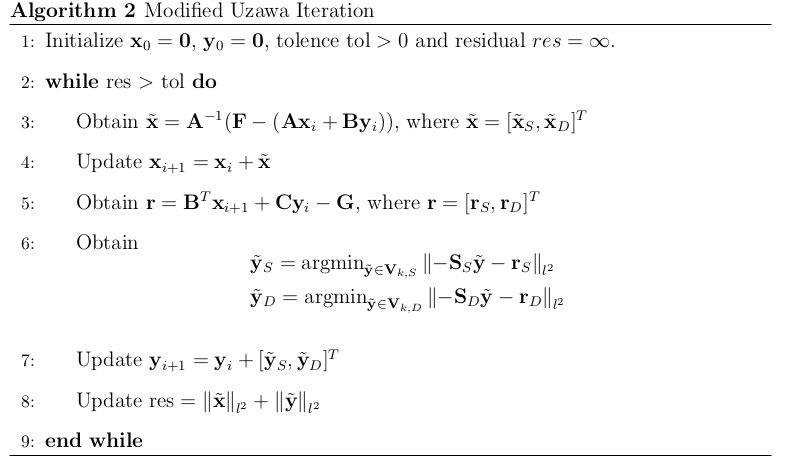
\includegraphics[width=15cm,height=9cm]{modified_Uzawa.png}

\end{myslide}

\begin{myslide}
\heading{Mid-ocean ridge case}
\centering
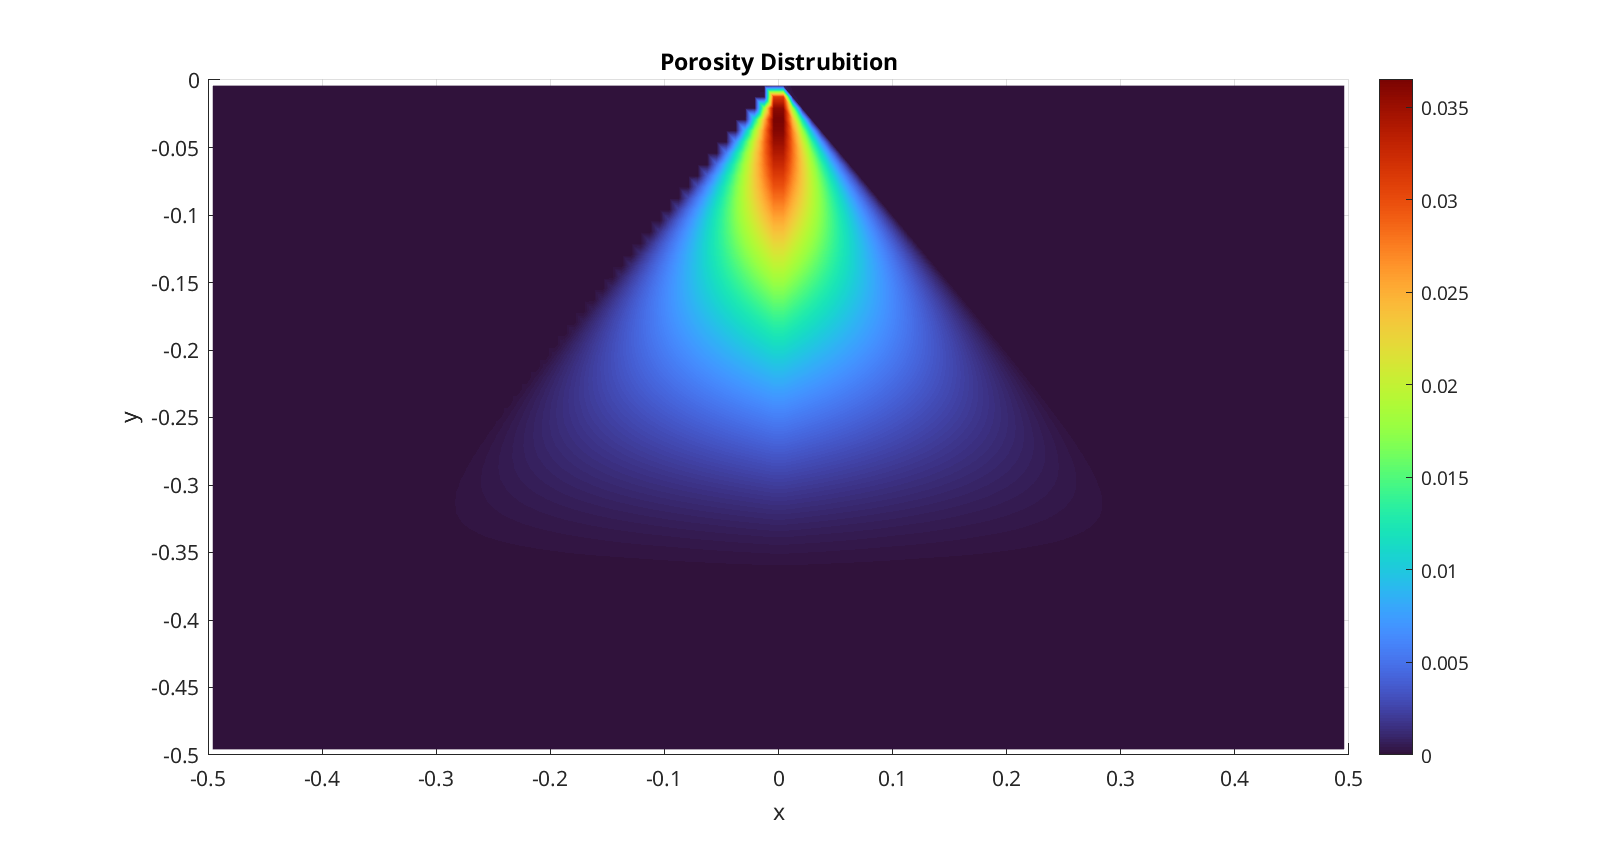
\includegraphics[width=16cm,height=8cm]{../formal/chapters/pics/mor_poro.eps}
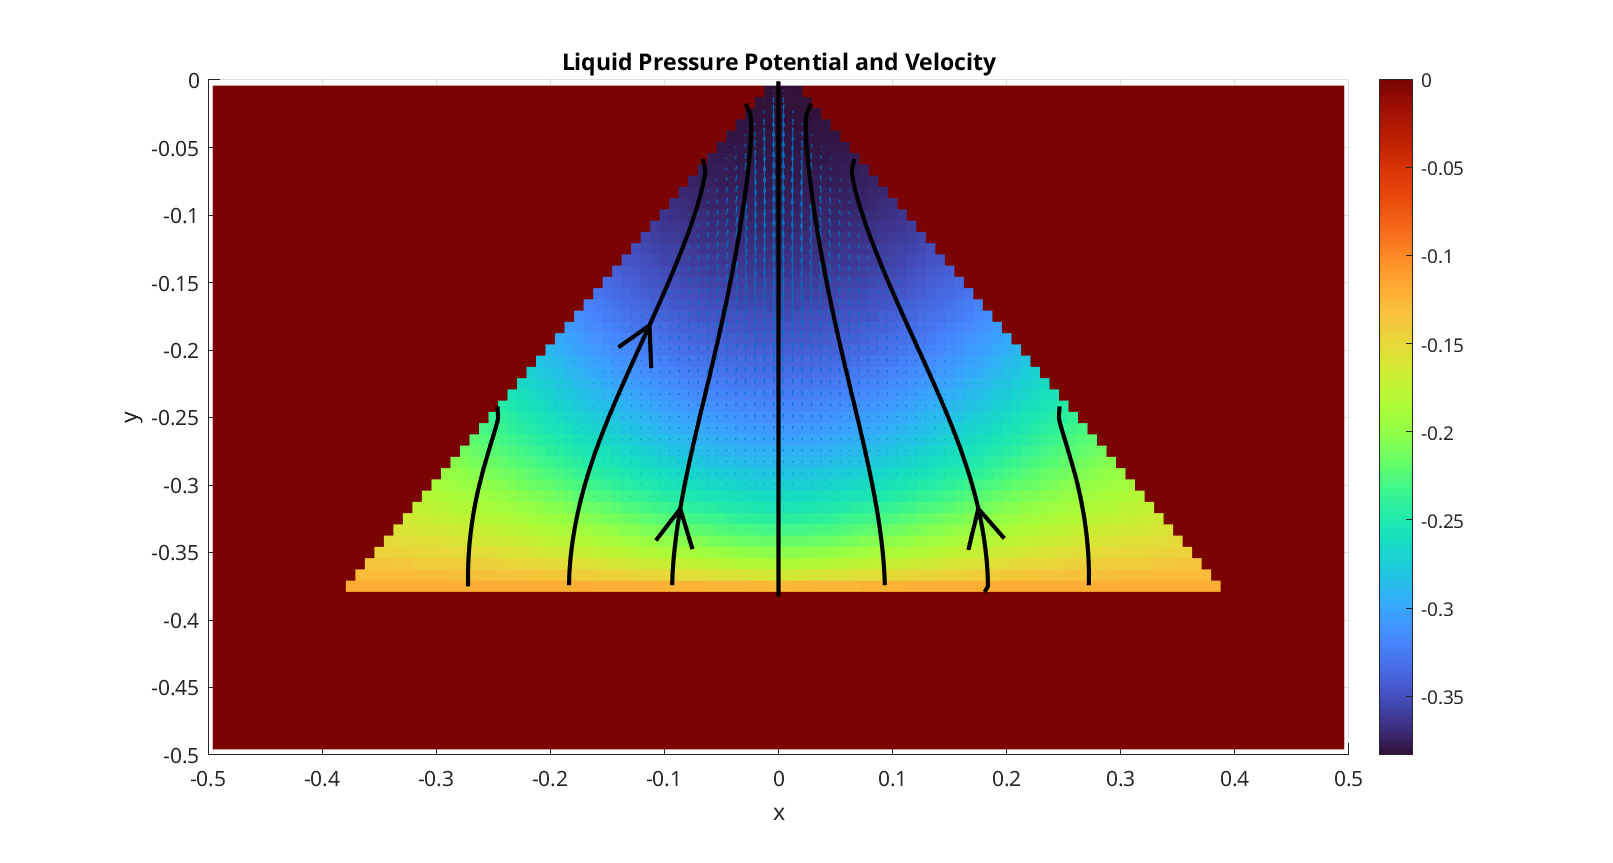
\includegraphics[width=16cm,height=8cm]{../formal/chapters/pics/mor_l.eps}
\end{myslide}

\begin{myslide}
\vspace{50pt}
\centering
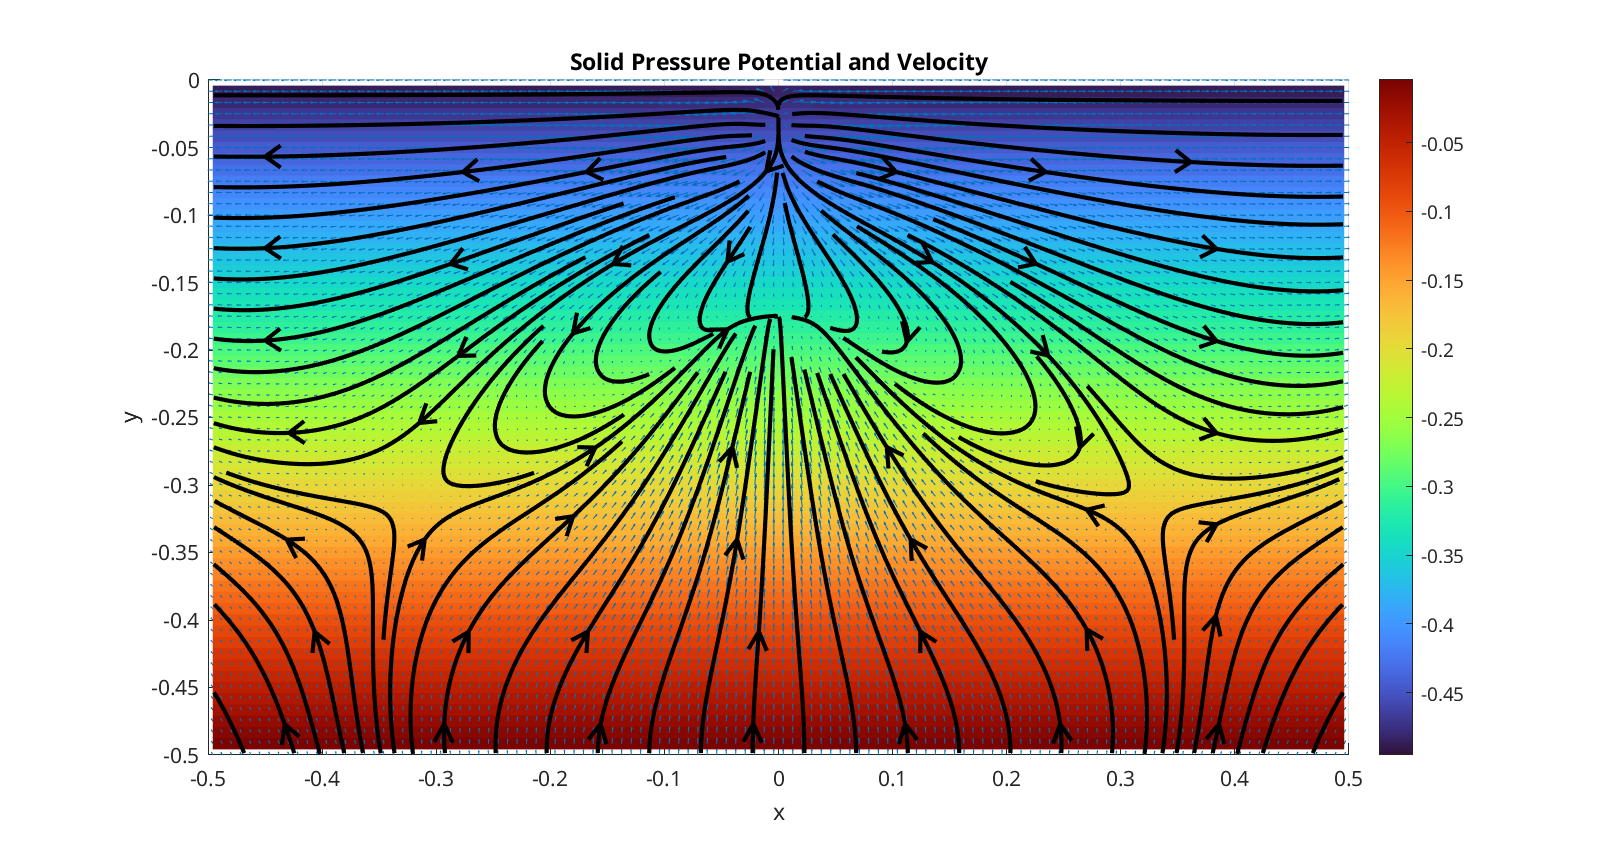
\includegraphics[width=25cm,height=12.5cm]{../formal/chapters/pics/mor_s.eps}
\end{myslide}

\begin{myslide}

\heading{Finite volume method}

\Oblue{General hyperbolic conservation law}:

\begin{equation}\label{eq:conservationlaw}
		  \left \{
		  \begin{alignedat}{2}
					 &\frac{\partial u(\mathbf{x},t)}{\partial t} + \nabla \cdot \mathbf{f}(u; \mathbf{x},t) = 0, \hspace{0.2cm} t>0,\, &&\mathbf{x} \in \Omega, \\ 
					 &u(\mathbf{x},0) = u_0(\mathbf{x}), \hspace{2.5cm} &&\mathbf{x} \in \Omega,
		  \end{alignedat}
		  \right .
\end{equation}

\vspace{20pt}

\Oblue{Semi-discretized form}:

\begin{equation}
		  \frac{\partial \overline{u}_E}{\partial t} + \frac{1}{\lvert E \rvert}\int_{\partial E} \mathbf{F}(\mathbf{x},t) \cdot \pmb{\nu}\, d\mathbf{x} = 0,
\end{equation}

\vspace{20pt}

\Oblue{Semi-discretized form with reconstructed value}:

\begin{equation}\label{eq:fvdis}
		  \frac{\partial \overline{u}_{E}}{\partial t} + \sum_{i=0}^4\frac{\lvert e_i \rvert}{\lvert E \rvert}
		  \sum_{g=0}^G \omega_{i,g} \mathbf{F}(\mathcal{R}_{i,g}^+, \mathcal{R}_{i,g}^-)\cdot \pmb{\nu}_i = 0,
\end{equation}

\end{myslide}

% ================================================

\begin{myslide}
\heading{Stencil Polynomials}
\Oblue{Scaled stencil polynomials}:

\begin{equation} \label{eq:stencilpolynomial}
		  Q^{\mathcal{S}}_{s,t}(x,y) = \sum_{p<s,\  q<t} c_{p,q} \Big(\frac{x - x_\mathcal{S}}{h_\mathcal{S}}\Big)^p 
		  \Big(\frac{y - y_\mathcal{S}}{h_\mathcal{S}}\Big)^q.
\end{equation}

\vspace{20pt}

\Oorange{Basis polynomials}:

\begin{equation}\label{eq:basispoly}
		  \frac{1}{\lvert E_{i',j'}\rvert } \iint_{E_{i',j'}} \phi^{i,j}_{s,t} (x,y)\, dxdy = 
		  %\frac{1}{\lvert \hat{E}_{k'}\rvert} \iint_{\hat{E}_{k'}}\hat{\phi}^k_{s,t}(\xi, \eta) d\xi d\eta = 
		  \left \{
					 \begin{aligned}
								&1 \quad  (i',j') = (i,j)\\
								&0 \quad  (i',j') \neq (i,j)
					 \end{aligned}
					 \right. 
					 ,\quad \forall E_{i',j'} \in \mathcal{S}.
\end{equation}

\vspace{20pt}

\Oblue{Rewrite with basis polynomials}:

\begin{equation}\label{eq:normalizedstencilpoly}
\hat{Q}^{\mathcal{S}}_{s,t}(\xi, \eta) = \sum_{i,j} \overline{u}_k \hat{\phi}_{s,t}^{i,j}(\xi, \eta).
\end{equation}

\end{myslide}

\begin{myslide}
\heading{Smoothness indicators}

\Oblue{Jiang-Shu smoothness indicator}:

\begin{equation}\label{eq:JSsmoothnessIC}
\begin{aligned}
		  \sigma_{JS} &= \sum_{1\leq \lvert \alpha \rvert \leq r}  \frac{h_\mathcal{S}^{2\lvert\alpha\rvert}}{\lvert E_0 \rvert} 
		  \iint_{E_0} (\mathcal{D}^\alpha Q(x,y))^2 dx dy\\
					  &= \frac{h_\mathcal{S}^2}{\lvert E_0 \rvert}\sum_{1\leq \lvert \alpha \rvert \leq r} \iint_{\hat{E}_0} (\mathcal{D}^\alpha\hat{Q}(\xi, \eta))^2 d\xi d\eta \\
					  &= \frac{h_\mathcal{S}^2}{\lvert E_0 \rvert}\sum_{1\leq \lvert \alpha \rvert \leq r} \iint_{\hat{E}_0} \big( \sum_{ij} \overline{u}_{ij} \mathcal{D}^\alpha \hat{\phi}_{i,j}(\xi, \eta) \big)^2 d\xi d\eta \\
					  &= \frac{h_\mathcal{S}^2}{\lvert E_0 \rvert}\sum_{ij} \sum_{i'j'} \overline{u}_{ij} \overline{u}_{i'j'} \sum_{1\leq \lvert \alpha \rvert \leq r} 
					  \iint_{\hat{E}_{ij}} \mathcal{D}^\alpha \hat{\phi}_{ij}(\xi, \eta) 
					  \mathcal{D}^\alpha \hat{\phi}_{i'j'}(\xi, \eta) d\xi d\eta \\
					  &= \frac{h_\mathcal{S}^2}{\lvert E_0 \rvert}\sum_{ij} \sum_{i'j'} \overline{u}_{ij} \overline{u}_{i'j'} \sigma^{i'j'}_{ij},
\end{aligned}
\end{equation}

\end{myslide}

\begin{myslide}

\vspace{20pt}

\begin{itemize}
\item \textit{\Oblue{Simple smoothness indicator}}%~\cite{WENOAOSimplifiedSmoothness}
\begin{equation}\label{eq:simpsmoothnessIC}
\sigma_{\text{simp}} = \frac{1}{N_\mathcal{S} -1 } \sum_k (\overline{u}_k - \overline{u}_0)^2,
\end{equation}
where $\overline{u}_0$ is the cell averaged solution in the target cell.
This simple smoothness indicator is designed to reduce the computational cost and to deal with
distorted stencils on unstructured meshes. However, this simple smoothness indicator is not as robust
as the classic Jiang-Shu smoothness indicator.

\vspace{20pt}

\item \textit{\Oblue{Polynomial smoothness indicator}}%~\cite{sigmaP}
		  \begin{equation}\label{eq:polysigma}
					 \sigma_{P} = \sum_{\alpha} \zeta_{\alpha, \alpha} c_{\alpha}^2
		  \end{equation}
		  which is obtained by dropping all the cross terms appeared in the formulation~\eqref{eq:cofformulation}.
		  This alternative serves as a good approximation to the classic Jiang-Shu smoothness indicator while the 
		  computing efficiency is greatly improved.
\end{itemize}

\end{myslide}

\begin{myslide}
\heading{ML-WENO Weighting}

\begin{equation}\label{eq:reconstruction}
\mathcal{R}(\mathbf{x}) = \sum_{l} \tilde{\omega_l} Q^{\mathcal{S}_l}(\mathbf{x}), \quad \mathbf{x} \in E_{i,j},
\end{equation}

\begin{equation}\label{eq:nonlinearwgts}
\hat{\omega}_l = \frac{\omega_l}{(\sigma_l + \epsilon h_0^2)^{ar_l + n_l}},
\end{equation}

\Oblue{Biasing factor}:

\begin{equation}\label{eq:biasingfctor}
n(r_l) = n_l = \begin{cases}
1, \quad &\text{if} \quad r_l = 1,\\
3, \quad &\text{if} \quad r_l = 2,\\
4, \quad &\text{if} \quad r_l \geq 3.
\end{cases}
\end{equation}

\Oblue{Renormalized scaling weights}:

\begin{equation}\label{eq:normalizednonlinearwgts}
\tilde{\omega}_l = \frac{\hat{\omega}_l}{\sum_{l'} \hat{\omega}_{l'}}.
\end{equation}

\end{myslide}

\begin{myslide}
\heading{Identifying shock}

\vspace{50pt}
\centering
\input ../formal/chapters/tikz/stencilsplit.tex

\end{myslide}

\begin{myslide}
\heading{Error Estimation}

\vspace{50pt}

\begin{lemma}
		  Let $\mathcal{R}(\mathbf{x})$ be the reconstruction. Assuming a 
		  qusi-uniform mesh, $h_0 = \Theta(h)$, there exists a constant $C>0$
		  such that for any $\mathbf{x} \in E_0$, 
		  \begin{equation}\label{eq:errorestimate}
					 \lvert u(\mathbf{x}) - \mathcal{R}(\mathbf{x}) \rvert \leq C h^{r_{\max}},
		  \end{equation}
		  where $r_{\max}$ is defined as $\max(r_x, r_y)$.
\end{lemma}

\end{myslide}

\begin{myslide}

\heading{Time stepping}

\vspace{50pt}

A multi-stage explicit SSP Runge-Kutta  method:
\begin{equation}\label{eq:multistageSSP}
\begin{aligned}
		  u^{0} &= u^n ,\\
		  u^{(i)}   &= \sum_{j=0}^{i-1} \alpha_{i,j}u^{(j)} + \Delta t \beta_{i,j} \tilde{\mathbf{F}}(u^{(j)}), \quad 1\leq i \leq m\\
		  u^{n+1} &= u^m,
\end{aligned}
\end{equation}
where $\sum_{j}^{i-1} \alpha_{i,j} = 1$.

\end{myslide}

\begin{myslide}
\heading{Reconstruction example}

\begin{equation}
u(x,y) = \left \{ 
		  \begin{alignedat}{2}
		  &\sin(x) \cos(y)  \quad && x\leq 0.5,\\
		  &\sin\bigg(\frac{(x+0.3)\pi}{2}\bigg)^6 \cos\bigg(\frac{(y-0.6)\pi}{2}\bigg)^6 + 0.5  \quad && x>0.5.
		  \end{alignedat}
		  \right.
\end{equation}

\vspace{50pt}
\centering
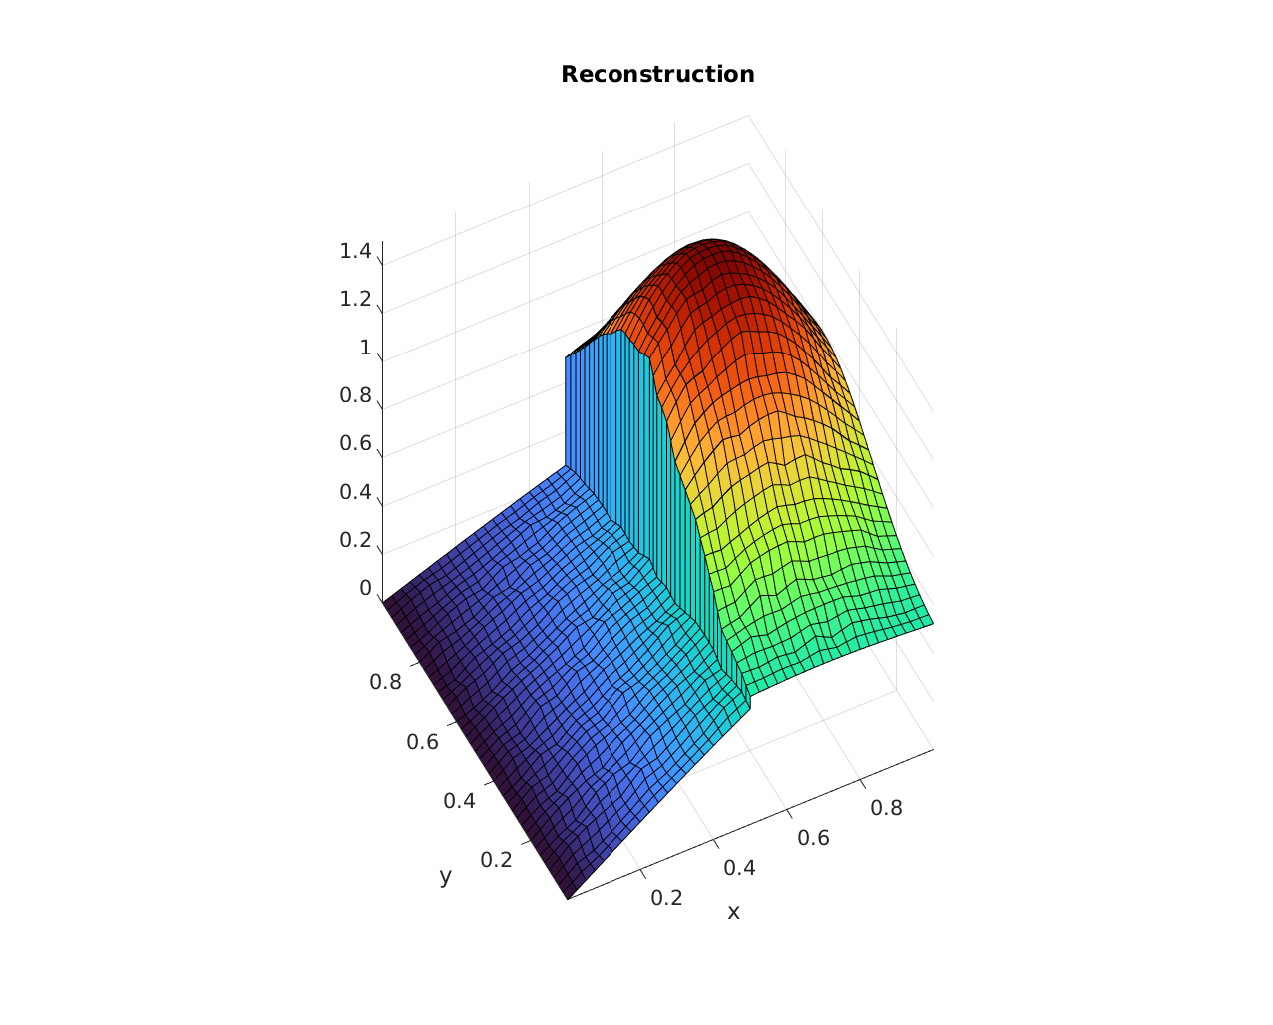
\includegraphics[width=20cm, height=11cm]{../formal/chapters/pics/53reconstruction.eps}

\end{myslide}

\begin{myslide}
		  \heading{Inflow boundary stabilization}
\begin{equation}
\label{eq:inflowtest}
u_D(0,y,t) = \left\{\begin{alignedat}{2}
&\sin^2(2\pi y),\quad &&y\leq0.25, y\geq 0.75,\\
&1,             \quad &&0.25 < y < 0.75.
\end{alignedat}
\right.
\end{equation}

		  \vspace{50pt}

\centering
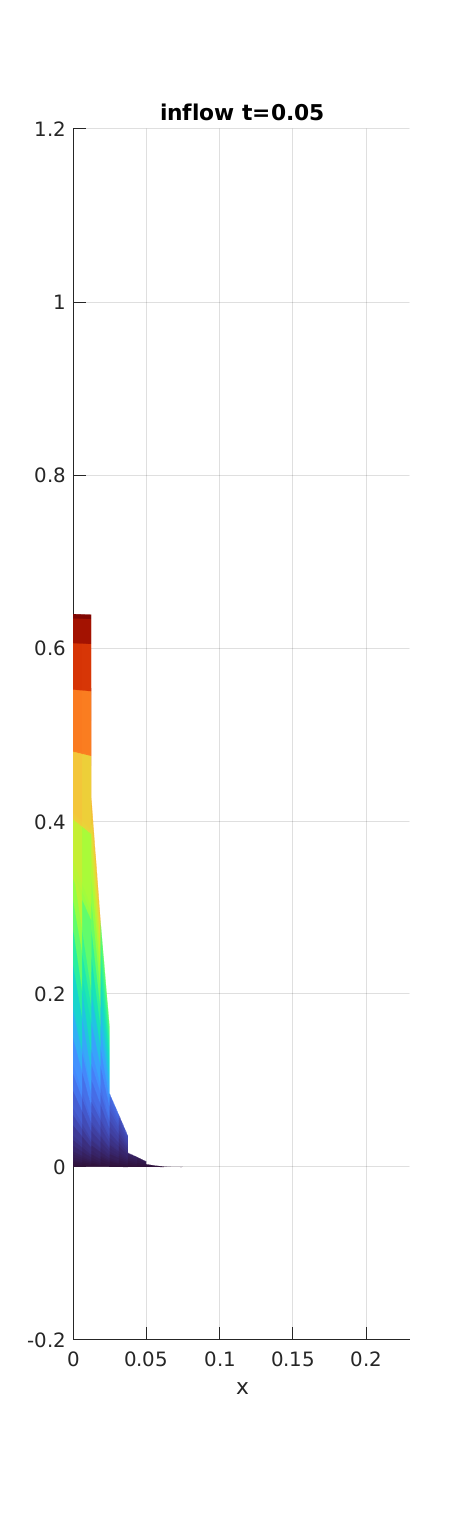
\includegraphics[width=4cm, height=10cm]{../formal/chapters/pics/newinflow005.eps}
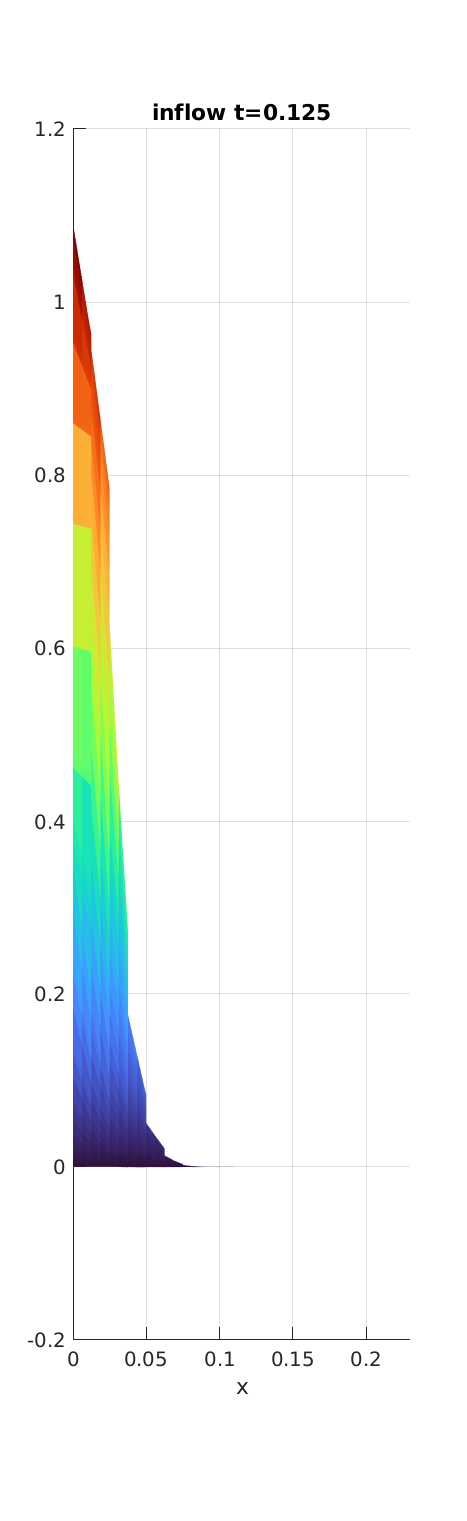
\includegraphics[width=4cm, height=10cm]{../formal/chapters/pics/newinflow0125.eps}
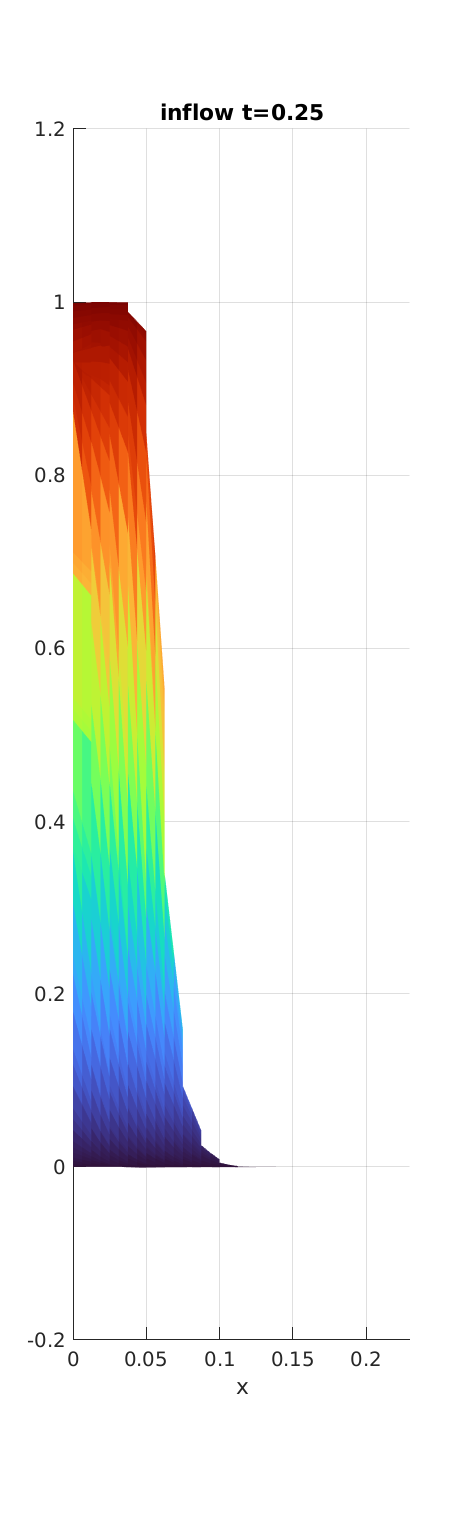
\includegraphics[width=4cm, height=10cm]{../formal/chapters/pics/newinflow025.eps}
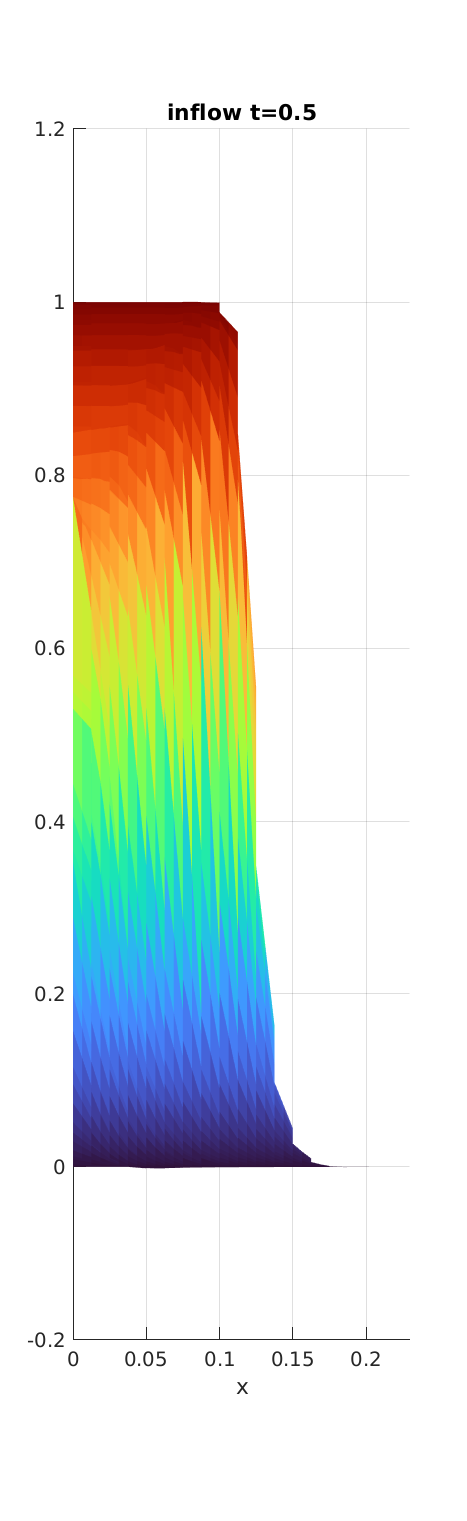
\includegraphics[width=4cm, height=10cm]{../formal/chapters/pics/newinflow05.eps}
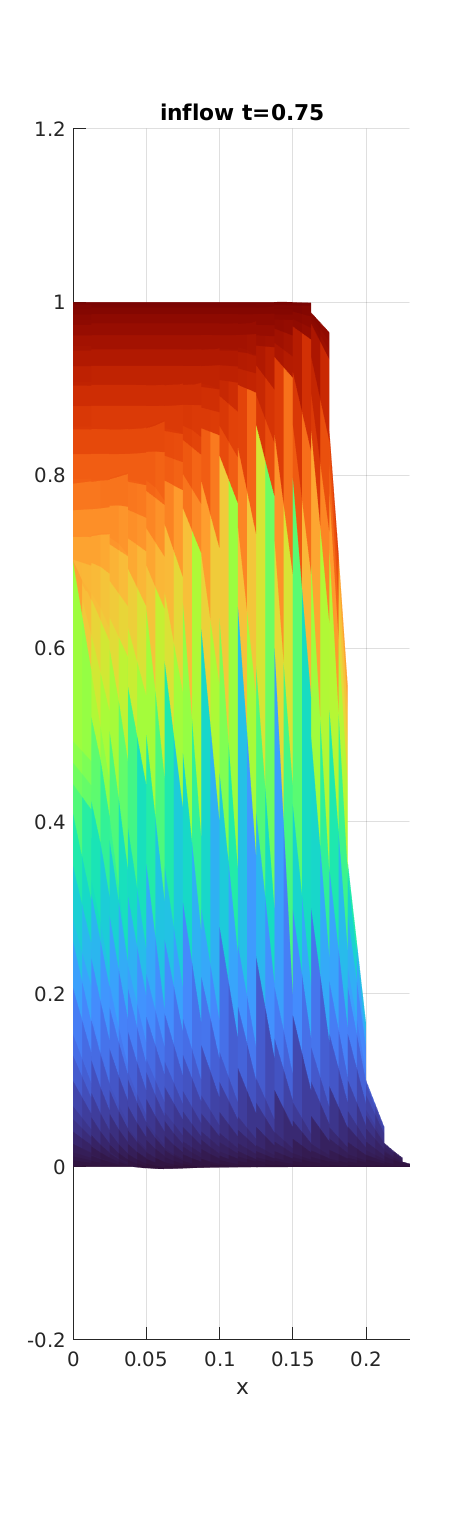
\includegraphics[width=4cm, height=10cm]{../formal/chapters/pics/newinflow075.eps}

\end{myslide}

\begin{myslide}
		  \heading{Rarefaction example}

\begin{equation}\label{eq:truesolutionrarefaction}
u(x,y,t) = \left \{ 
\begin{aligned}
&0, \hspace{2.2cm} x<0.5, x\geq 0.5t+1.5,\\
&(x-0.5)/t,\hspace{0.5cm} 0.5\leq x <t+0.5,\\
&1, \hspace{2.2cm} t+0.5 \leq x < 0.5t+1.5.
\end{aligned}
		  \right.
\end{equation}

\centering
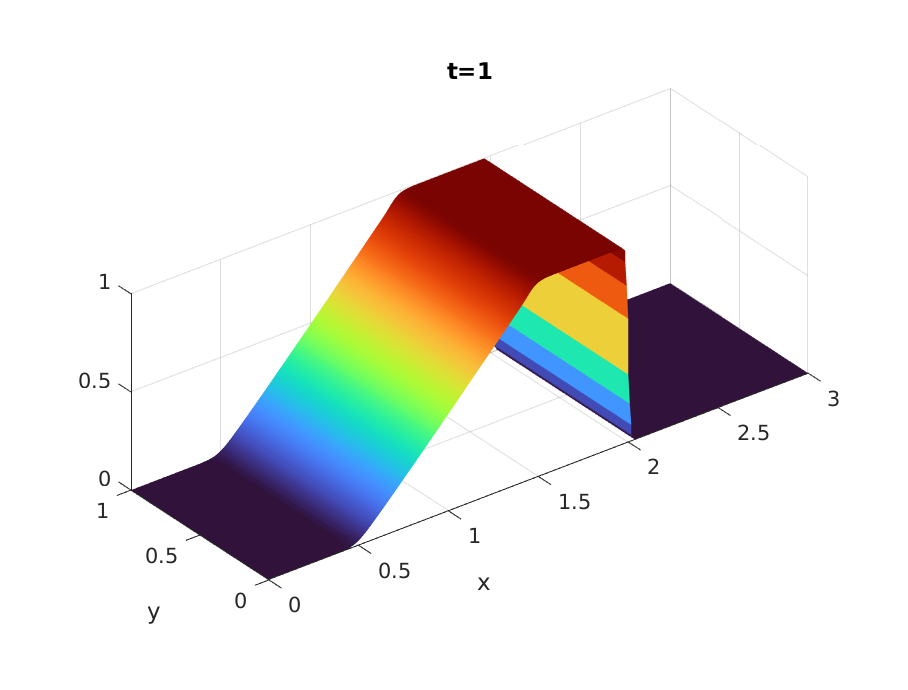
\includegraphics[width=12cm,height=10cm]{../formal/chapters/pics/rarefraction_1.eps}
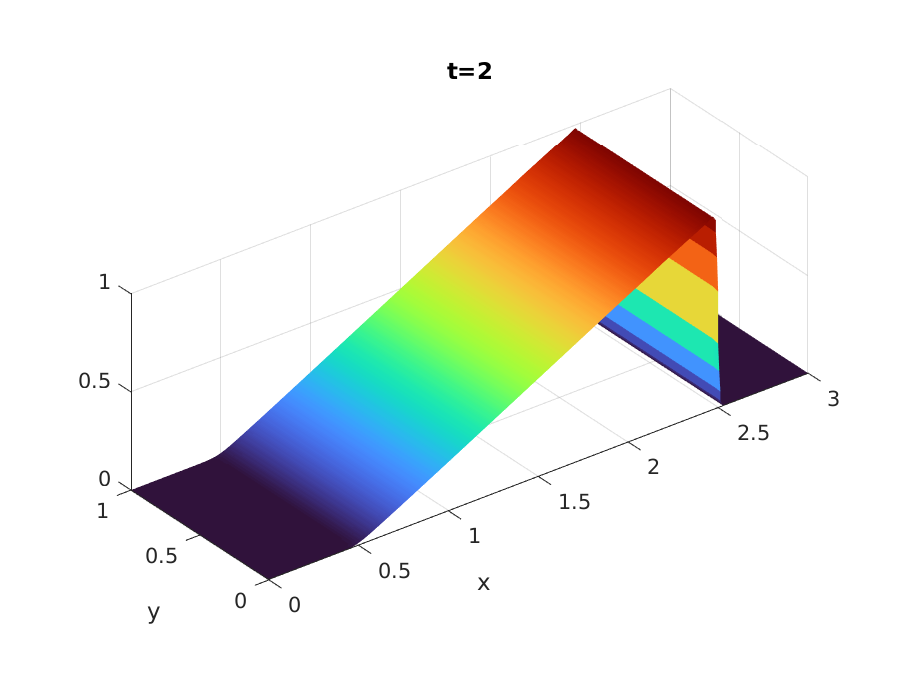
\includegraphics[width=12cm,height=10cm]{../formal/chapters/pics/rarefraction_2.eps}

\end{myslide}

\separatorHeading{\outno Let's couple them together}

\begin{myslide}
\heading{Coupled Solver}

\vspace{50pt}

\centering
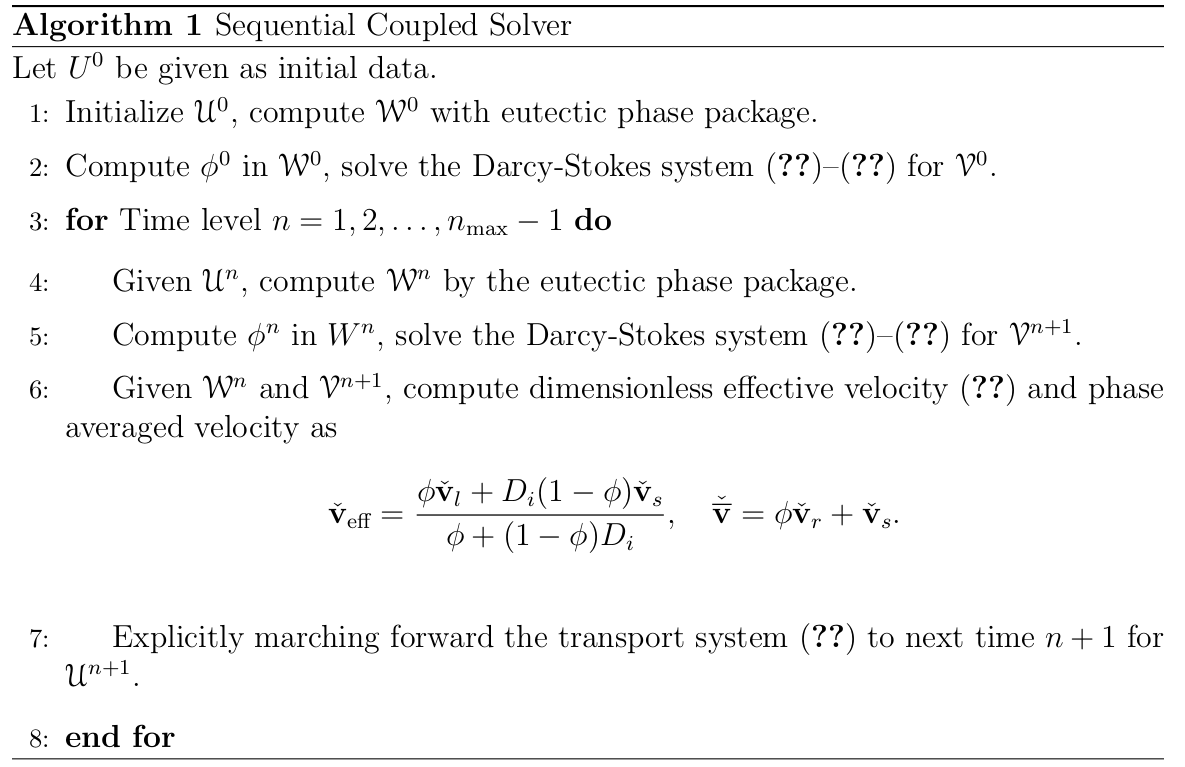
\includegraphics[width=22cm,height=15cm]{coupled_algo.png}

\end{myslide}

\begin{myslide}

\heading{Simplified Case}

\centering
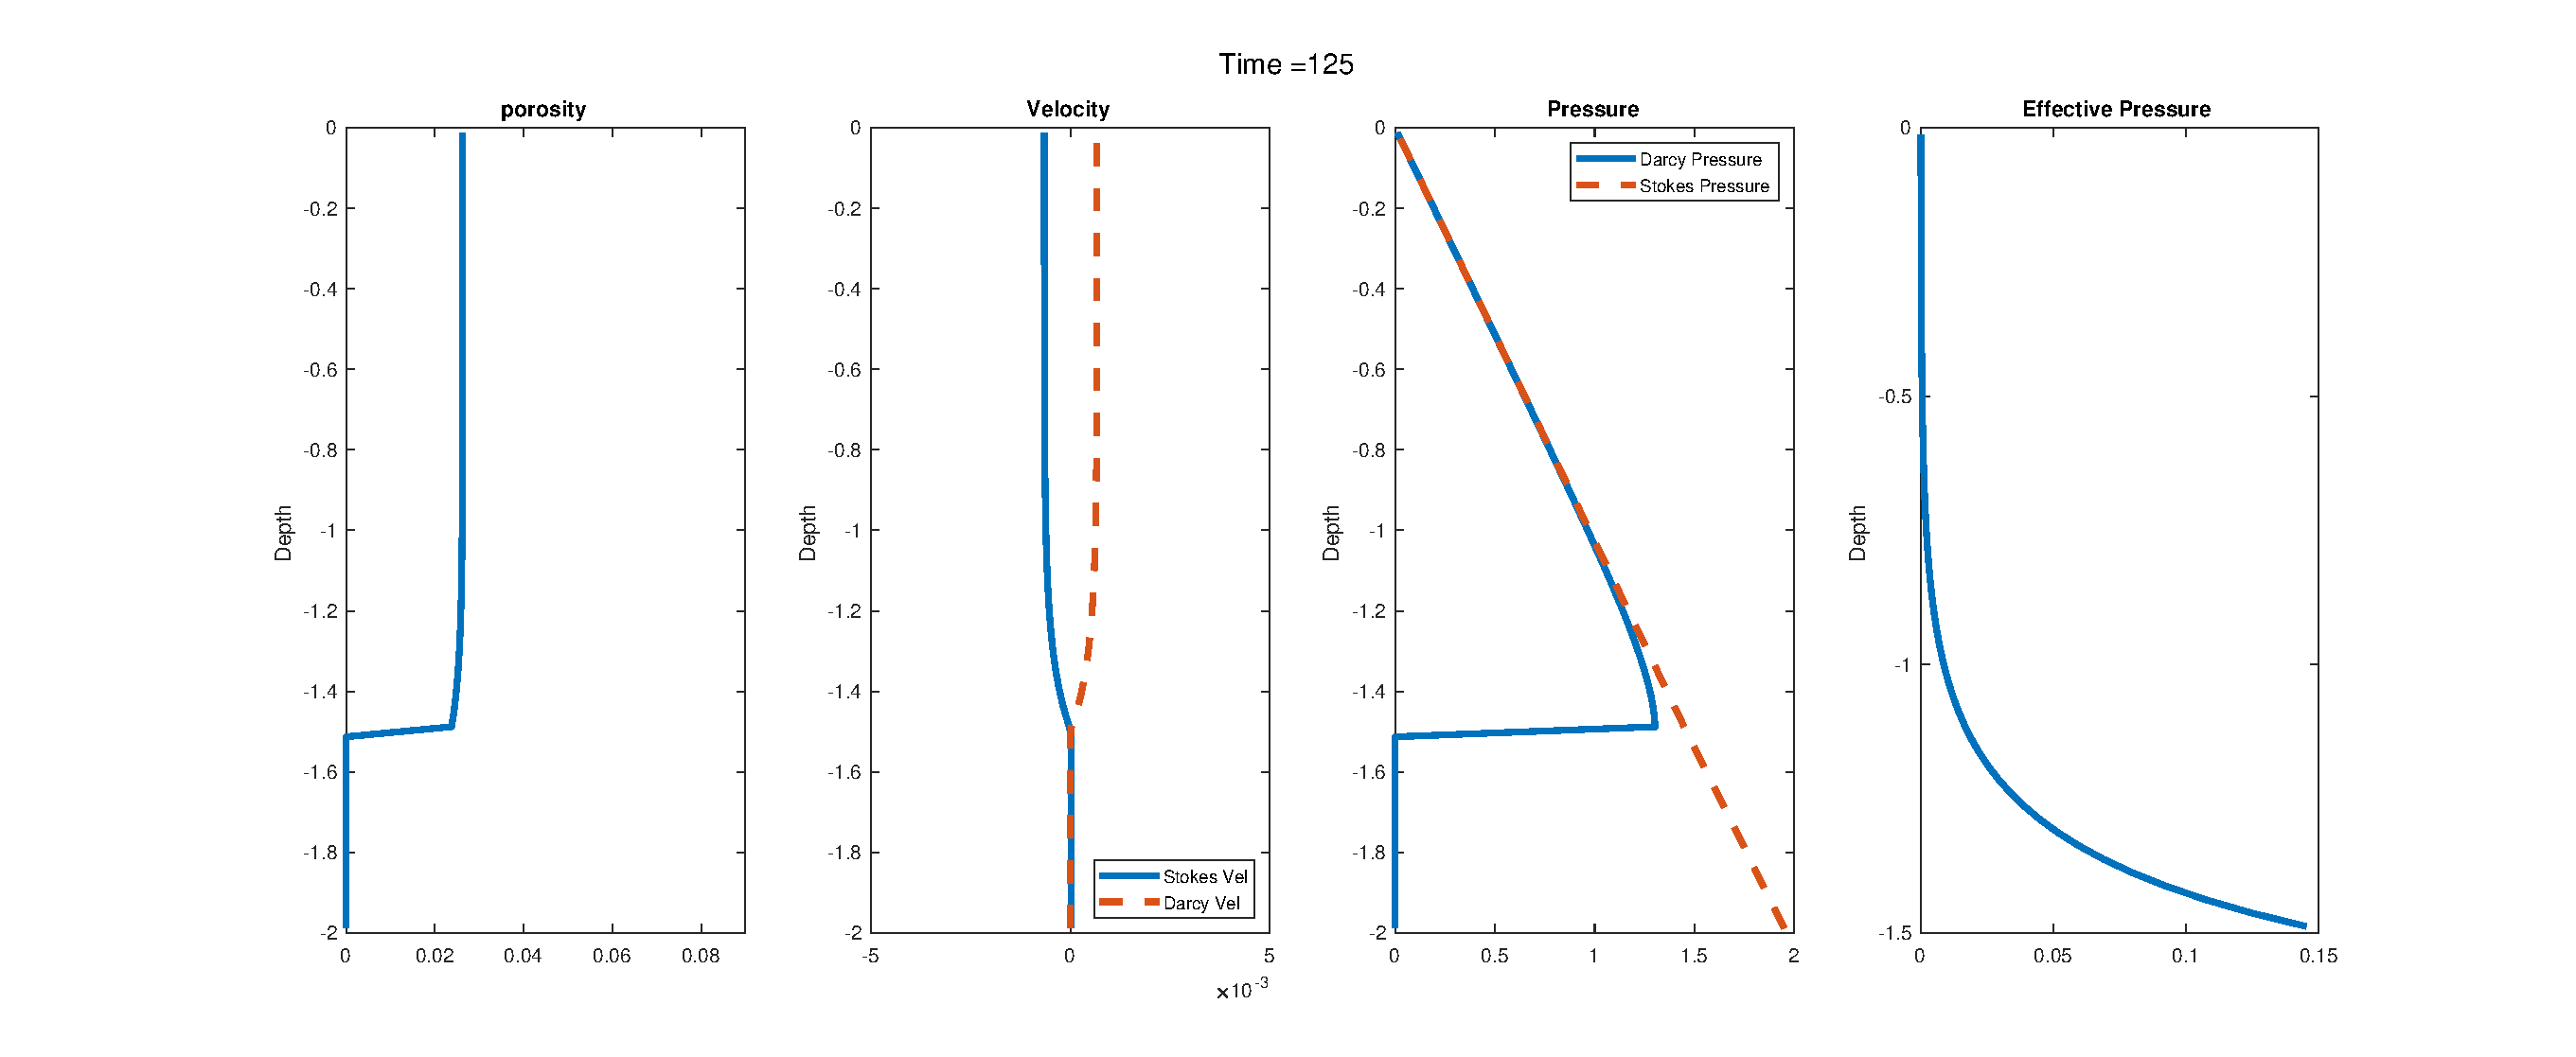
\includegraphics[width=14cm,height=6.5cm]{../formal/chapters/pics/constmelt_t125.eps}
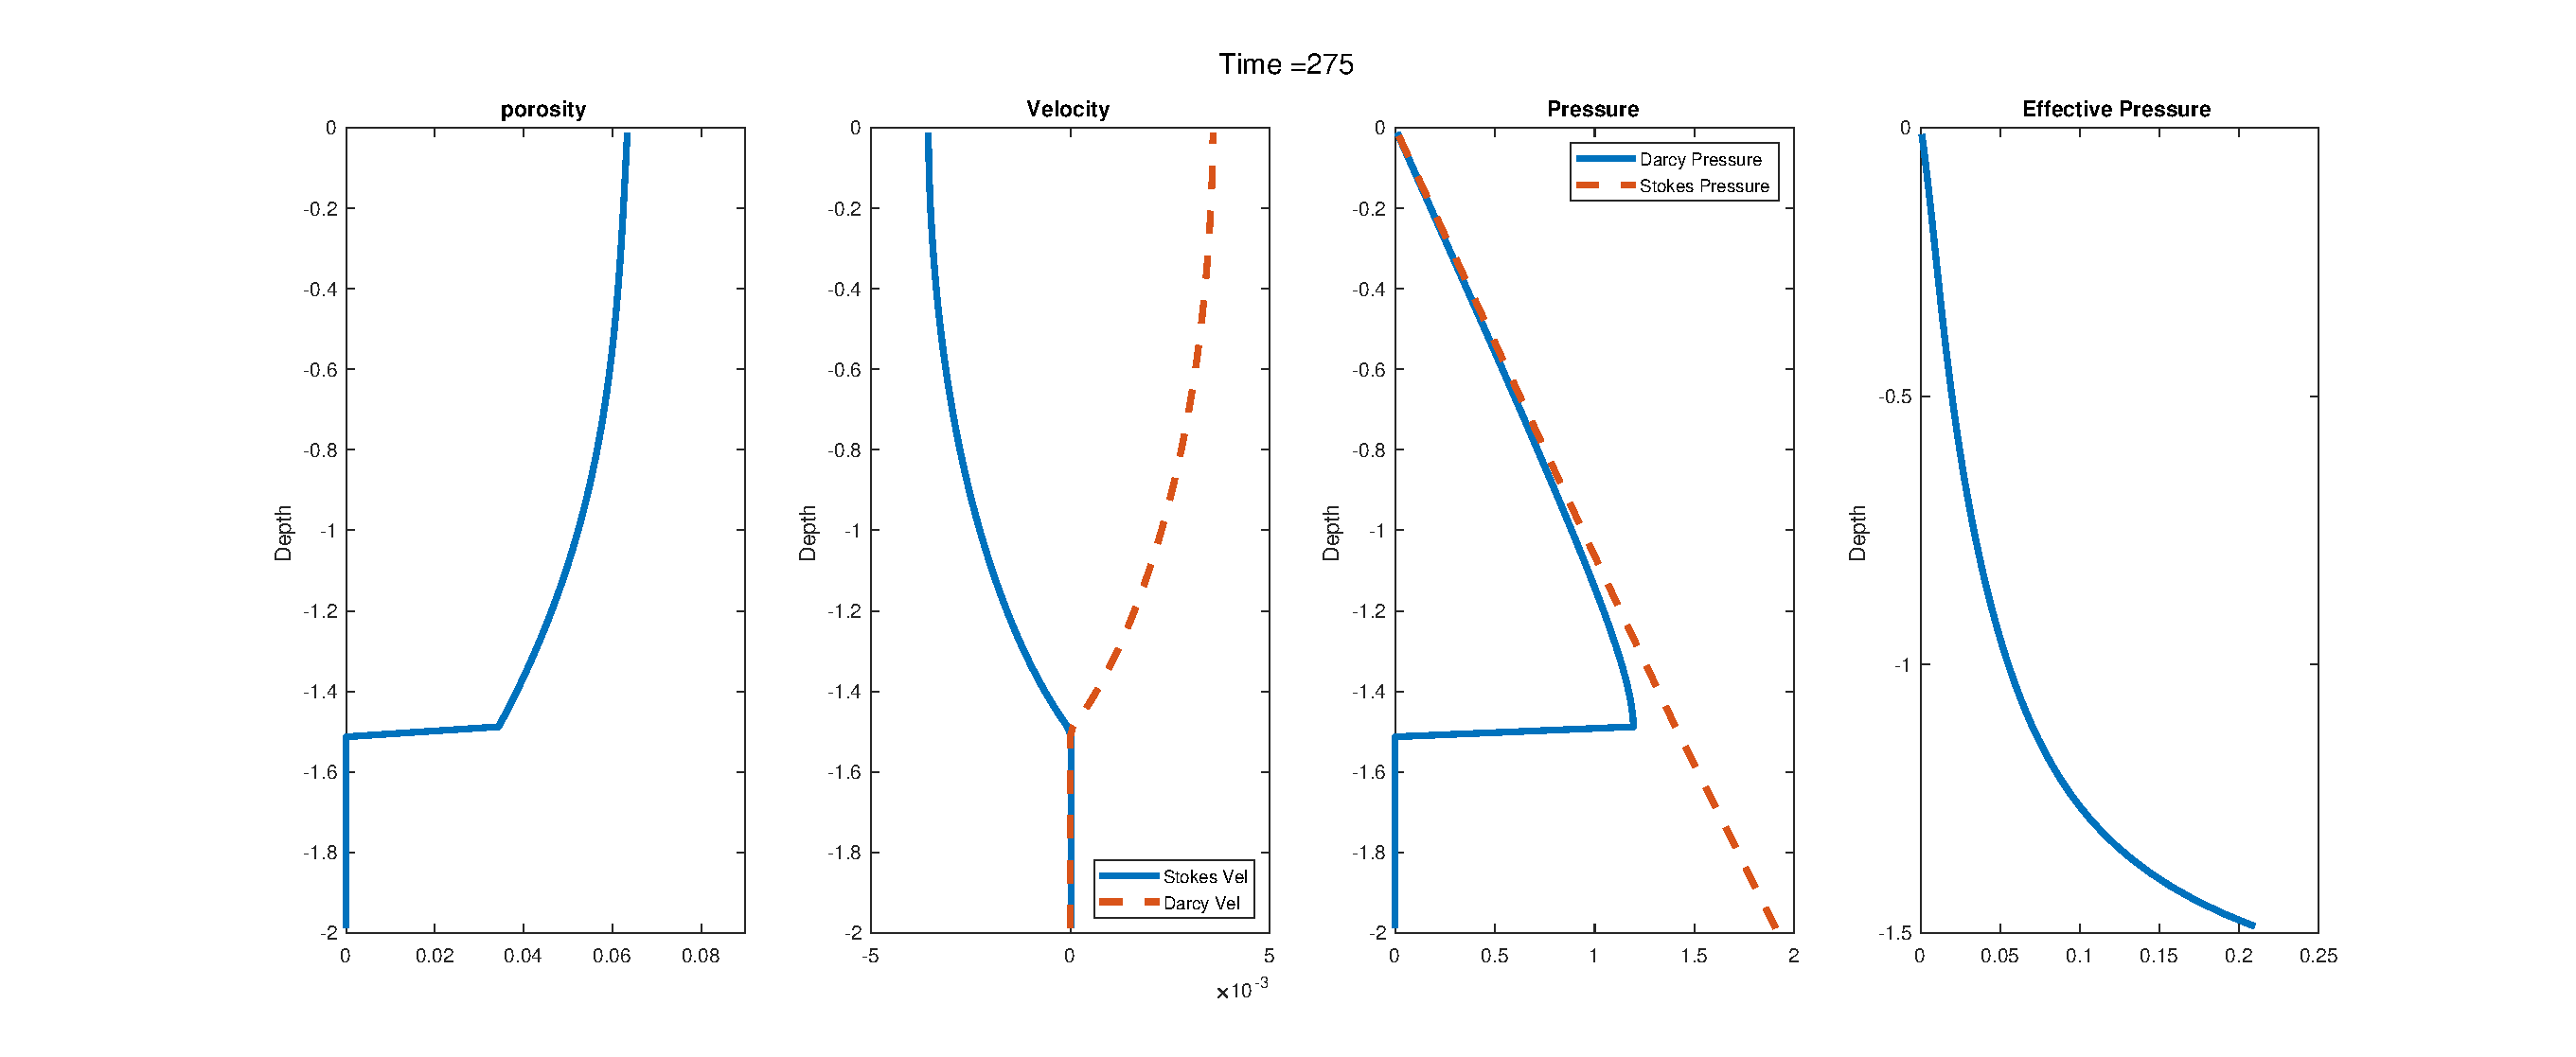
\includegraphics[width=14cm,height=6.5cm]{../formal/chapters/pics/constmelt_t275.eps}
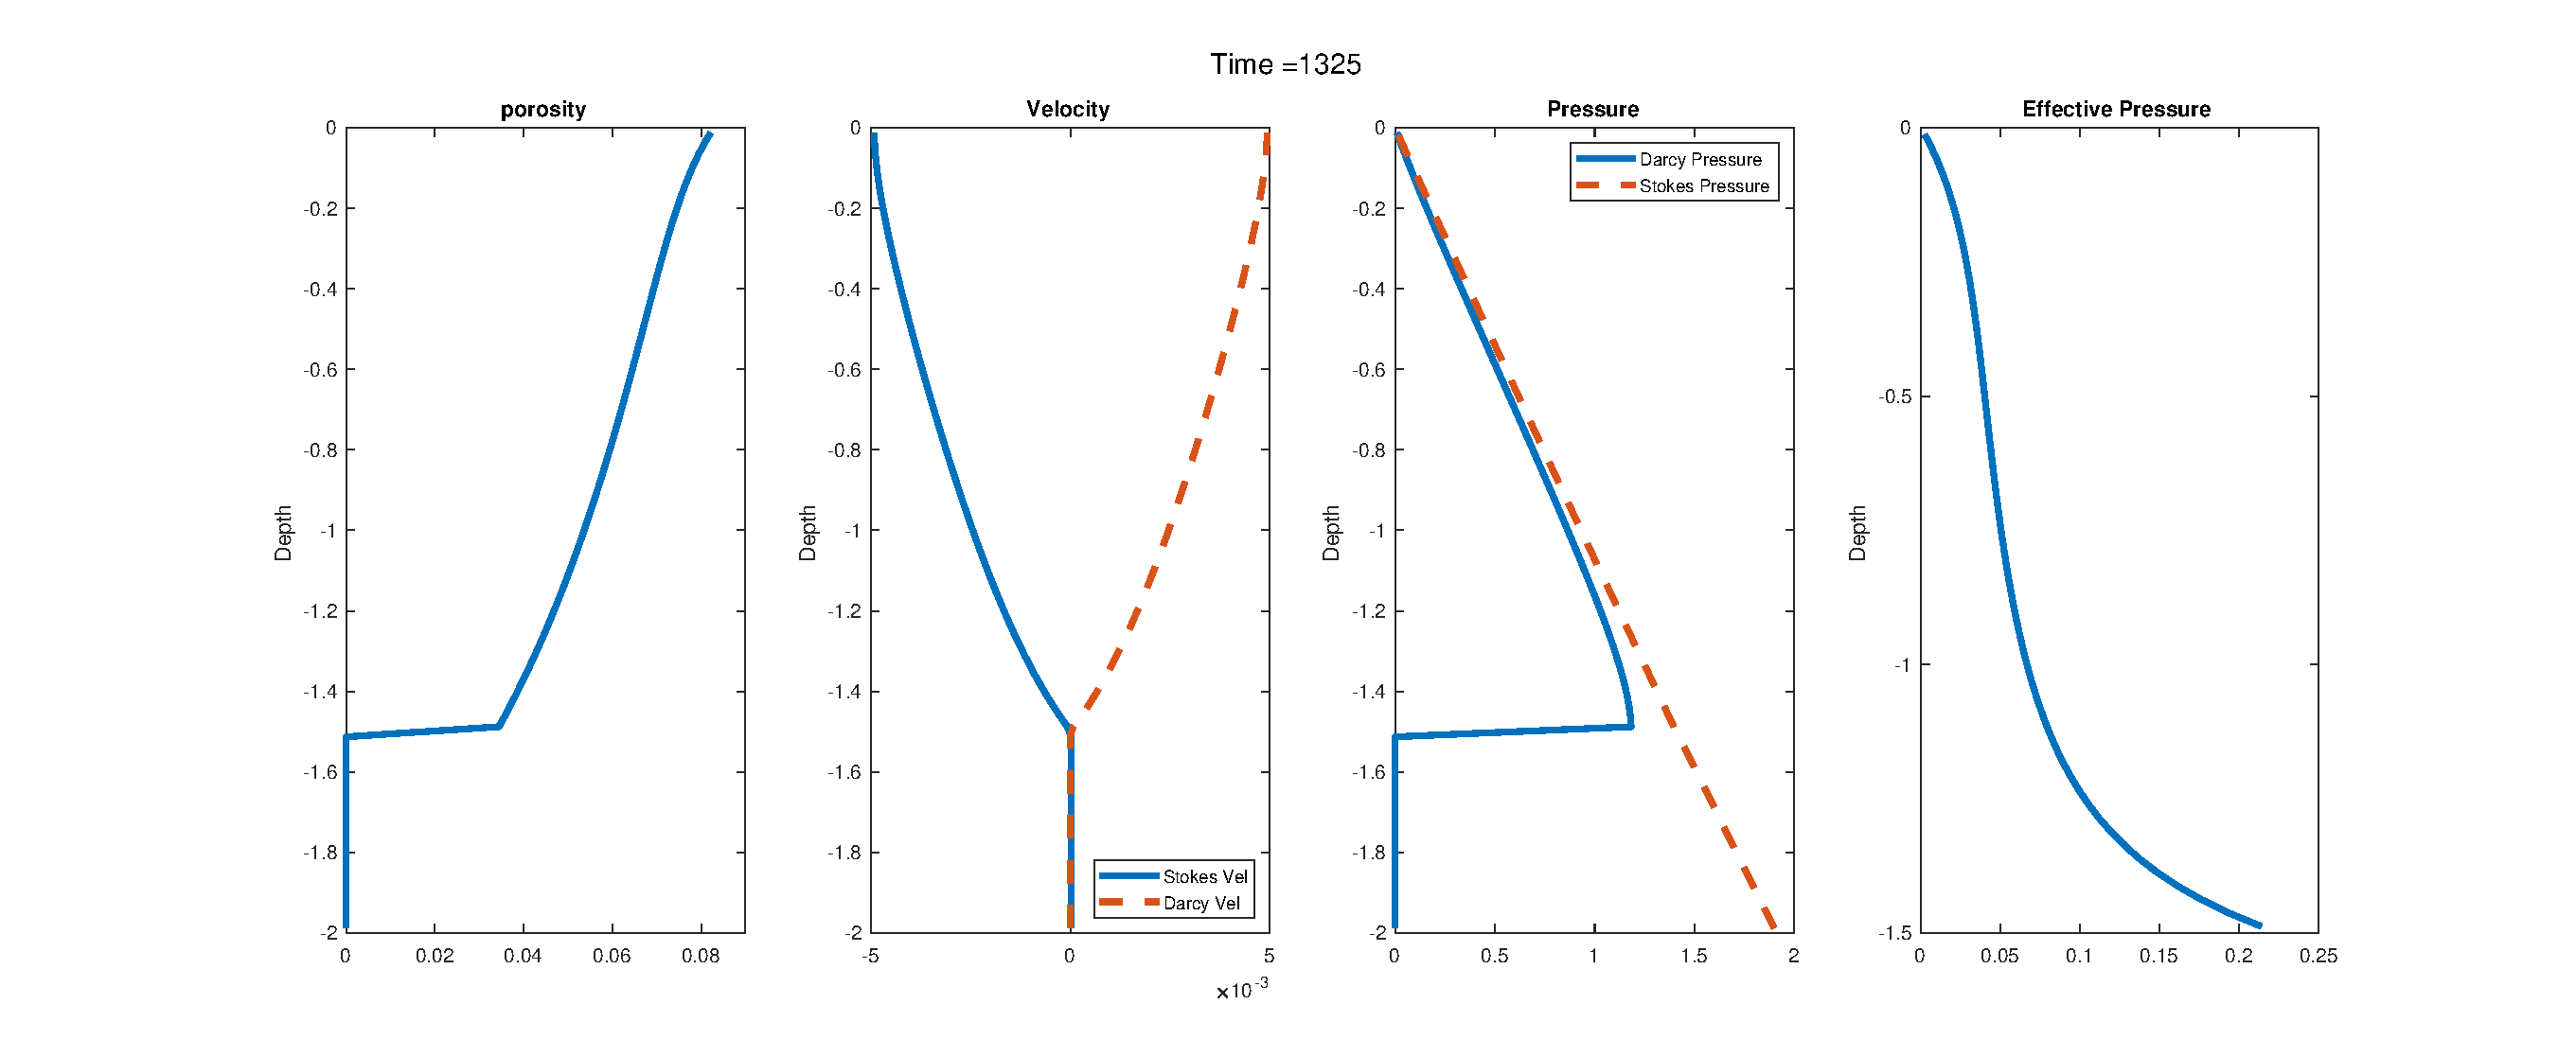
\includegraphics[width=14cm,height=6.5cm]{../formal/chapters/pics/constmelt_t1325.eps}

\end{myslide}

\begin{myslide}

Let's see some videos.

\end{myslide}

\end{document}
